% TEMPLATE — {{TOKENS}} are filled by `python -m src.reporting.report`. Edit this file, not ieee_report.tex.
% Compile ieee_report.tex with pdfLaTeX (e.g. on Overleaf). Figures are read from figures/ (or ../../artifacts/figures/).
\documentclass[conference]{IEEEtran}
\usepackage{graphicx,booktabs,amsmath,amssymb,url}
\usepackage[hidelinks]{hyperref}
\graphicspath{{figures/}{../figures/}{../../artifacts/figures/}}

\begin{document}
\title{Predicting Which MCP Tool Descriptions Cause Agent Errors: An Explainable Machine Learning Framework for Detecting High-Risk Model Context Protocol Tool Descriptions}
\author{\IEEEauthorblockN{Student Name(s) --- Roll No(s).}
\IEEEauthorblockA{Department of Computing -- AI \& ML, Coimbatore Institute of Technology, Coimbatore\\19MAM56 Advanced Machine Learning Lab -- CAT II Project}}
\maketitle

\begin{abstract}
AI agents act on external systems through Model Context Protocol (MCP) tools, which they understand only through a name, a natural-language description and a JSON input schema. Poorly written definitions make agents select the wrong tool, omit required arguments or send invalid values. We frame tool-definition risk as a supervised learning problem. We assemble 2181 MCP-format tool records (1579 real Berkeley Function-Calling Leaderboard functions with real user queries and gold calls, 99 MCP reference-server tools and 503 documented augmentations) and label every tool with a controlled agent benchmark (10 simulated episodes, BFCL-style call validation). A 169-dimensional fusion of TF-IDF/LSA text features, MiniLM sentence embeddings, JSON-schema statistics and engineered risk scores feeds 14 models; XGBoost and LightGBM are tuned with Optuna under grouped cross-validation. The selected XGBoost (Optuna-tuned) reaches test PR-AUC 0.709 (95\% CI [0.624, 0.793]), ROC-AUC 0.779 and F1 0.684, against 0.406 for a no-skill baseline and 0.416 for a documentation-quality heuristic. Feature fusion adds +0.033 PR-AUC over the best single feature family. SHAP explanations drive actionable recommendations, and the system is served by a validated FastAPI service, containerised with Docker and publicly deployed on Hugging Face Spaces.
\end{abstract}
\begin{IEEEkeywords}Model Context Protocol, function calling, LLM agents, explainable AI, SHAP, gradient boosting, Optuna\end{IEEEkeywords}

\section{Introduction}
\textbf{Problem.} The Model Context Protocol (MCP)~\cite{mcp,mcpsurvey} standardises how large language model (LLM) agents discover and call external tools. An agent sees each tool only as a triple $t=(n,d,s)$: a name $n$, a free-text description $d$ and an input JSON schema $s$. From this text alone it must choose the right tool for a request and build a valid call. When the description is vague, parameters are undocumented or untyped, or the schema is deeply nested, agents route requests to the wrong tool, omit required arguments, hallucinate parameters or send values in the wrong format.

\textbf{Motivation and impact.} Tool catalogues are written by many authors and rarely reviewed. Failures surface only at run time, where they waste tokens, trigger retries and can cause incorrect actions in real systems. A \emph{pre-deployment} risk score that also explains \emph{why} a definition is risky lets maintainers fix documentation before any agent sees it.

\textbf{Research question.} \emph{Can the probability that a tool definition causes agent errors be predicted from the definition alone, and can the prediction be explained in actionable terms?}

\textbf{Objectives.} (i) Build a reproducible, provenance-labelled dataset of MCP tool definitions with measured failure labels; (ii) engineer text, semantic and structural features with dimensionality reduction; (iii) benchmark baselines against advanced, Optuna-tuned models with significance testing, ablation and error analysis; (iv) explain predictions with SHAP and turn them into recommendations; (v) deploy a validated inference service and dashboard with Docker and a public cloud endpoint.

\section{Literature Review}
\textbf{Tool-augmented LLMs.} Toolformer~\cite{toolformer} showed that language models can learn when to call APIs, and ReAct~\cite{react} interleaves reasoning traces with tool actions. ToolLLM~\cite{toolllm} scaled tool use to more than 16{,}000 real REST APIs, and Gorilla~\cite{gorilla} fine-tuned a model on API documentation and introduced AST-based call matching. The Berkeley Function-Calling Leaderboard (BFCL)~\cite{bfcl} turned this into a public benchmark of functions, user questions and gold calls, which we reuse as the backbone of our dataset.

\textbf{Documentation and agent success.} Hsieh \emph{et al.}~\cite{hsieh} showed that tool documentation alone enables zero-shot tool use, and EasyTool~\cite{easytool} improved agent success by rewriting verbose documentation into concise instructions. Hou \emph{et al.}~\cite{mcpsurvey} survey the MCP ecosystem and its risks. These works treat documentation as an \emph{intervention} that changes agent behaviour.

\textbf{Research gap.} Within the literature we surveyed, no work \emph{predicts} tool-level failure risk from the definition itself before deployment, explains that prediction, and validates it against measured call failures. Consequently there is no published numeric benchmark for this exact task; we therefore compare against a no-skill baseline, a documentation-quality heuristic and a matrix of 14 learned models, with paired significance tests (Section~\ref{sec:results}).

\textbf{Methods used.} Gradient-boosted trees (XGBoost~\cite{xgb}, LightGBM~\cite{lgbm}) are strong learners on fused tabular features; Sentence-BERT~\cite{sbert} with a MiniLM backbone~\cite{minilm} gives compact semantic embeddings; UMAP~\cite{umap} supports visual inspection of embedding space; Optuna~\cite{optuna} provides efficient hyperparameter search; SHAP~\cite{shap} gives additive, model-consistent explanations. Because failures are the minority, costly class, we follow~\cite{davis,saito} and use PR-AUC as the primary metric, with bootstrap confidence intervals~\cite{efron}.

\section{Methodology}
\begin{figure*}[t]\centering\includegraphics[width=0.78\textwidth]{00_methodology.png}\caption{MCPGuard methodology: data collection, controlled labelling, preprocessing, feature engineering and reduction, modelling and tuning, explainability, error analysis and deployment.}\label{fig:method}\end{figure*}
Fig.~\ref{fig:method} shows the end-to-end pipeline; every stage is a Python module run by one command, and all reported numbers are regenerated from its artefacts.

\subsection{Data sources and preprocessing}
We convert 1579 BFCL v3 functions~\cite{bfcl} (Apache-2.0, with real user questions and gold calls) and 99 tools from the MCP reference servers into a common MCP format. To cover the risky end of the distribution we add 503 variants produced by nine documented operators (e.g.\ vague description, stripped parameter descriptions, removed types or enums, malformed schema, and documentation \emph{enrichment}); every variant keeps the lineage of its seed tool. Preprocessing applies Unicode and whitespace normalisation, identifier splitting (\texttt{getUserName}~$\rightarrow$ ``get user name''), JSON-schema parsing with repair and type-alias normalisation, exact de-duplication (29 removed), near-duplicate grouping (379 groups) and median imputation. The 13 malformed schemas are \emph{kept and flagged}, because a broken schema is itself a risk signal. The result is 2152 clean records from 670 servers.

\subsection{Controlled agent benchmark (labels)}
For each tool, a documentation-bounded simulated agent runs $K=10$ episodes (real BFCL questions for 2050 tools, synthetic intents otherwise). Routing picks among the target, its co-loaded siblings and random distractors with an embedding softmax
\begin{equation}
p(j\mid q)=\frac{\exp\big(\cos(\mathbf{e}_q,\mathbf{e}_j)/T\big)}{\sum_{k}\exp\big(\cos(\mathbf{e}_q,\mathbf{e}_k)/T\big)},\quad T=0.02,
\end{equation}
where $\mathbf{e}$ are MiniLM embeddings of the request and tool texts. Arguments are then constructed with success probabilities that depend only on what the request and the documentation expose (e.g.\ 0.97 for a literal value in the request, 0.86 with a format hint, 0.55 for an undocumented parameter), and each call is validated BFCL-style against the hidden schema and gold values, yielding one of seven error types. With failure rate $r(t)=\frac1K\sum_{k=1}^{K}\mathbb{I}[\text{episode }k\text{ fails}]$, the binary target is
\begin{equation}
y(t)=\mathbb{I}\big[r(t)\ge\tau\big],\qquad \tau=0.30 .
\end{equation}
The mean episode failure is 27.4\% and the positive rate is 40.7\% (imbalance 1.454:1).

\subsection{Feature engineering and dimensionality reduction}
Each tool is mapped to a fused vector
\begin{multline}
\mathbf{x}(t)=\big[\,\mathrm{SVD}_{64}(\mathrm{TFIDF}(d))\;;\;\mathrm{PCA}_{48}(\mathrm{MiniLM}(d))\;;\\
\mathbf{s}_{26}\;;\;\mathbf{l}_{25}\;;\;\mathbf{r}_{6}\,\big]\in\mathbb{R}^{169}.
\end{multline}
TF-IDF uses word 1--2-grams (4{,}000 terms) and character 3--5-grams (3{,}000), reduced by truncated SVD (latent semantic analysis, $X\approx U_k\Sigma_kV_k^{\top}$) to 64 \emph{text themes} labelled by their top terms. all-MiniLM-L6-v2 embeddings (384-d) are reduced by PCA to 48 dimensions. $\mathbf{s}$ holds 26 schema statistics (parameter count, required ratio, nesting depth, untyped and enum counts, described ratio, \ldots), $\mathbf{l}$ 25 lexical statistics (length, vague-word rate, average word length, imperative and constraint cues, \ldots), and $\mathbf{r}$ six bounded risk scores, e.g.
\begin{align}
\text{ambiguity}&=\min\!\big(1,\;5v/\max(T_d,1)+0.5\,\mathbb{I}[T_d<6]\big),\\
\text{missing constraint}&=1-h/P,
\end{align}
where $v$ is the vague-word count, $T_d$ the token count, $h$ the number of parameters with type/format hints and $P$ the parameter count. UMAP~\cite{umap} and 2-D PCA are used only for visualisation (Fig.~\ref{fig:umap}).

\subsection{Models and objective}
We train logistic regression, random forest, histogram gradient boosting, an MLP, XGBoost and LightGBM. For gradient boosting with trees $f_k$, the regularised, class-weighted objective is
\begin{equation}
\mathcal{L}=\sum_{i} w_i\,\ell\big(y_i,\hat y_i\big)+\sum_{k}\Big(\gamma J_k+\tfrac12\lambda\|\boldsymbol\omega_k\|_2^2+\alpha\|\boldsymbol\omega_k\|_1\Big),
\end{equation}
with logistic loss $\ell$, $J_k$ leaves with weights $\boldsymbol\omega_k$, and $w_i=1.45$ for positives (the inverse class ratio). The experiment matrix E1--E6 crosses feature sets (TF-IDF, embeddings, fused) with learners, and benchmark models B0--B7 add a majority baseline, a documentation-quality rule and further learners. The decision threshold is $\theta^*=\arg\max_\theta \mathrm{F1}_{\text{val}}(\theta)$, and the production model is chosen on \emph{validation} PR-AUC, then F1, then ROC-AUC; the test split is used once.

\subsection{Hyperparameter search}
Optuna~\cite{optuna} with a TPE sampler and median pruning maximises mean average precision over 4-fold \texttt{StratifiedGroupKFold} on the training split. Table~\ref{tab:space} lists the search space (40 XGBoost and 30 LightGBM trials; 15 and 15 pruned).
\begin{table}[t]\centering\caption{Optuna search space (log = log-uniform)}\label{tab:space}
\resizebox{\columnwidth}{!}{\begin{tabular}{lll}\toprule
\textbf{Hyperparameter} & \textbf{XGBoost} & \textbf{LightGBM}\\\midrule
n\_estimators & 150--900 (step 50) & 150--900 (step 50)\\
max\_depth / num\_leaves & 2--9 & 8--96\\
learning\_rate & 0.01--0.25 (log) & 0.01--0.25 (log)\\
subsample & 0.55--1.0 & 0.55--1.0\\
colsample\_bytree & 0.3--1.0 & 0.3--1.0\\
min\_child\_weight / samples & 0.5--12 (log) & 5--60\\
gamma & $10^{-3}$--5 (log) & ---\\
reg\_alpha & $10^{-4}$--5 (log) & $10^{-4}$--5 (log)\\
reg\_lambda & $10^{-3}$--20 (log) & $10^{-3}$--20 (log)\\\bottomrule
\end{tabular}}\end{table}

\subsection{Evaluation, explainability and leakage control}
The 70/15/15 split (1537/307/308 tools; 1005/202/196 lineage groups) is stratified and \emph{grouped by lineage}, so near-duplicates and augmented variants of a tool never straddle splits. We report accuracy, precision, recall, F1, ROC-AUC, PR-AUC (average precision, $\mathrm{AP}=\sum_n (R_n-R_{n-1})P_n$), MCC, log-loss and Brier score, with 1{,}000-resample bootstrap 95\% CIs~\cite{efron} and paired bootstrap tests of $\Delta$PR-AUC against every baseline. SHAP TreeExplainer~\cite{shap} decomposes each prediction as $f(\mathbf{x})=\phi_0+\sum_j\phi_j$; tests verify that the SHAP values sum to the model logit. A rule layer maps the top positive SHAP drivers and schema issues to ranked recommendations.

\section{Implementation \& Experiments}
\textbf{Environment.} Python 3.14 on a CPU-only Windows PC with scikit-learn~\cite{sklearn}, XGBoost, LightGBM, sentence-transformers, Optuna, SHAP, UMAP and MLflow; global seed 42. The full pipeline (data $\rightarrow$ benchmark $\rightarrow$ features $\rightarrow$ tuning $\rightarrow$ 14 models $\rightarrow$ ablation $\rightarrow$ SHAP $\rightarrow$ figures $\rightarrow$ report) runs with one command in about 11 minutes. Every run is logged to MLflow (SQLite backend) and to an append-only JSONL log (16 tracked runs); 53 automated tests cover preprocessing, features, split leakage, the model contract, SHAP additivity and the API.

\textbf{Workflow.} (1) Build and label the dataset; (2) fit the feature pipeline on the training split only; (3) tune XGBoost and LightGBM with Optuna; (4) train E1--E6 and B0--B7 with identical splits; (5) select on validation and tune the threshold; (6) evaluate once on test with bootstrap CIs and paired tests; (7) run a feature-family ablation (5-fold grouped CV on train+val); (8) compute SHAP and error analysis.

\textbf{Model behaviour.} SHAP attributes Text (LSA) 44\%, Semantic embedding 29\%, Schema structure 14\%, Lexical / naming 8\%, Engineered risk scores 4\% of the mean $|\phi|$ to each feature family. The strongest global drivers are Schema size, Text theme \#23 (distance, untyped, search), Schema complexity score, Text theme \#45 (function, coordinates, longitude), Average word length (Fig.~\ref{fig:shap}). Fig.~\ref{fig:umap} shows that failing tools are spread across embedding space rather than forming one cluster, which is why semantic embeddings alone are not enough and structural features matter. The best XGBoost configuration (n\_estimators=600, max\_depth=5, learning\_rate=0.0142, subsample=0.771, colsample\_bytree=0.501, min\_child\_weight=0.728, gamma=0.00138, reg\_alpha=0.000516, reg\_lambda=0.0371) reached a grouped-CV PR-AUC of 0.690, against 0.685 for LightGBM.

\begin{figure}[t]\centering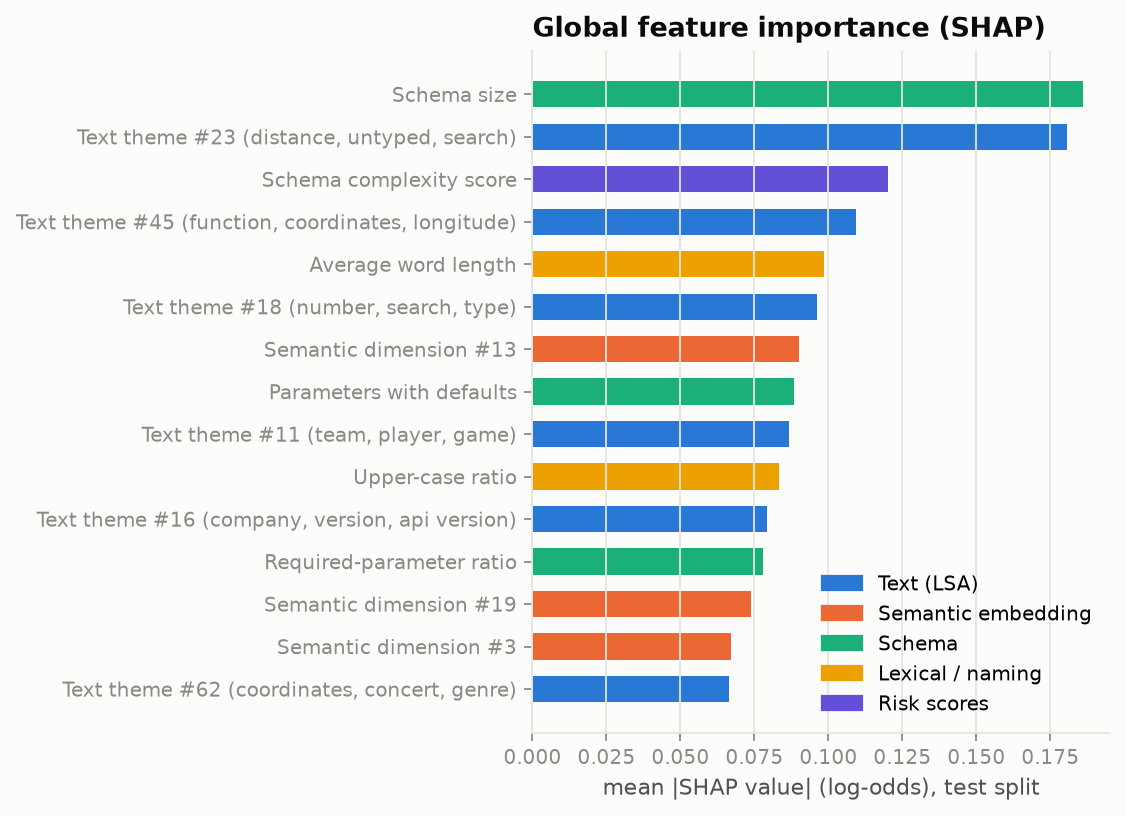
\includegraphics[width=\columnwidth]{04_shap_importance.png}\caption{Global SHAP importance (mean $|\phi|$, test split), coloured by feature family.}\label{fig:shap}\end{figure}
\begin{figure}[t]\centering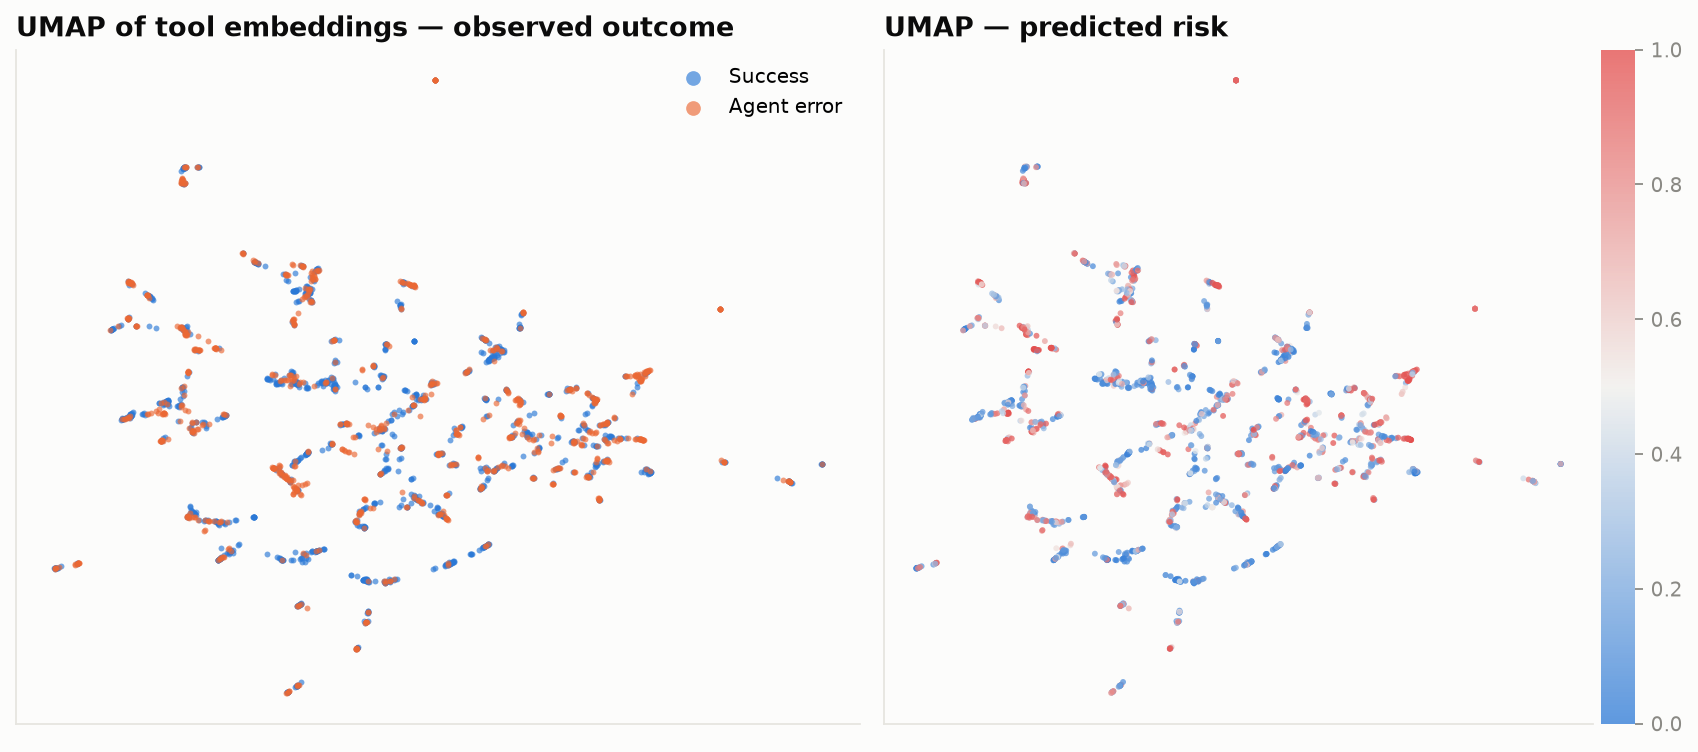
\includegraphics[width=\columnwidth]{06_umap_projection.png}\caption{UMAP projection of MiniLM tool embeddings: observed outcome (left) and predicted risk (right).}\label{fig:umap}\end{figure}

\section{Results \& Comparative Analysis}\label{sec:results}
\begin{table*}[t]\centering\caption{Held-out test benchmark, sorted by PR-AUC (selected production model in bold; selection used validation only)}\label{tab:bench}
\begin{tabular}{lrrrrrr}\toprule
\textbf{Model / features} & \textbf{Accuracy} & \textbf{Precision} & \textbf{Recall} & \textbf{F1} & \textbf{ROC-AUC} & \textbf{PR-AUC} \\ \midrule
Combined Features + MLP Neural Network & 0.604 & 0.507 & 0.928 & 0.655 & 0.800 & 0.745 \\
Combined Features + Random Forest & 0.744 & 0.672 & 0.720 & 0.695 & 0.783 & 0.711 \\
\textbf{Optimized Combined Features + XGBoost} & \textbf{0.724} & \textbf{0.639} & \textbf{0.736} & \textbf{0.684} & \textbf{0.779} & \textbf{0.709} \\
Combined Features + Logistic Regression & 0.718 & 0.617 & 0.800 & 0.697 & 0.803 & 0.706 \\
TF-IDF + Random Forest & 0.692 & 0.584 & 0.832 & 0.686 & 0.779 & 0.698 \\
Combined Features + XGBoost & 0.643 & 0.538 & 0.856 & 0.660 & 0.762 & 0.693 \\
Combined Features + LightGBM & 0.536 & 0.464 & 0.928 & 0.619 & 0.750 & 0.692 \\
Optimized Combined Features + LightGBM & 0.594 & 0.500 & 0.880 & 0.638 & 0.763 & 0.690 \\
Combined Features + Hist. Gradient Boosting & 0.506 & 0.447 & 0.912 & 0.600 & 0.735 & 0.676 \\
TF-IDF + Logistic Regression & 0.601 & 0.505 & 0.824 & 0.626 & 0.735 & 0.661 \\
Semantic Embedding + Random Forest & 0.640 & 0.544 & 0.696 & 0.611 & 0.695 & 0.616 \\
Semantic Embedding + XGBoost & 0.617 & 0.520 & 0.728 & 0.607 & 0.673 & 0.599 \\
Doc-quality heuristic (rule) & 0.406 & 0.405 & 0.984 & 0.573 & 0.492 & 0.416 \\
Majority / prior baseline & 0.406 & 0.406 & 1.000 & 0.577 & 0.500 & 0.406 \\
\bottomrule\end{tabular}\end{table*}

\textbf{Comparative analysis.} Table~\ref{tab:bench} compares all 14 models. The selected XGBoost (Optuna-tuned) reaches PR-AUC 0.709 (95\% CI [0.624, 0.793]), ROC-AUC 0.779 ([0.726, 0.828]), F1 0.684 ([0.615, 0.743]), precision 0.639, recall 0.736, specificity 0.716 and MCC 0.445, with log-loss 0.561 and Brier score 0.187. It clearly beats the no-skill baseline (0.406) and the documentation-quality heuristic (0.416), and the TF-IDF + logistic regression text baseline (0.661). Table~\ref{tab:paired} shows that the gains over the heuristic and over embedding-only models are significant (CI excludes zero), whereas several fused-feature learners are statistically tied. In particular, the MLP has the highest \emph{test} PR-AUC, but its difference from the selected model is not significant; choosing it on the test split would be test-set selection, so we keep the validation-selected model.

\begin{table}[t]\centering\caption{Paired bootstrap of test PR-AUC: selected model minus baseline (1{,}000 resamples)}\label{tab:paired}
\resizebox{\columnwidth}{!}{\begin{tabular}{llrlr}\toprule
\textbf{ID} & \textbf{Baseline} & \textbf{$\Delta$PR-AUC} & \textbf{95\% CI} & \textbf{p} \\ \midrule
B1 & Doc-quality heuristic (rule) & +0.289 & [+0.188, +0.377] & 0.000 \\
E4 & Semantic Embedding + XGBoost & +0.110 & [+0.053, +0.166] & 0.000 \\
E3 & Semantic Embedding + Random Forest & +0.092 & [+0.045, +0.142] & 0.000 \\
E1 & TF-IDF + Logistic Regression & +0.048 & [-0.014, +0.111] & 0.074 \\
B5 & Combined Features + Hist. Gradient Boosting & +0.033 & [+0.007, +0.061] & 0.003 \\
B7 & Optimized Combined Features + LightGBM & +0.021 & [-0.002, +0.045] & 0.044 \\
B4 & Combined Features + LightGBM & +0.018 & [-0.008, +0.047] & 0.086 \\
E5 & Combined Features + XGBoost & +0.017 & [-0.010, +0.045] & 0.103 \\
E2 & TF-IDF + Random Forest & +0.011 & [-0.035, +0.053] & 0.315 \\
B2 & Combined Features + Logistic Regression & +0.004 & [-0.058, +0.063] & 0.428 \\
B3 & Combined Features + Random Forest & -0.002 & [-0.027, +0.024] & 0.563 \\
B6 & Combined Features + MLP Neural Network & -0.034 & [-0.084, +0.019] & 0.913 \\
\bottomrule\end{tabular}}\end{table}

\begin{figure}[t]\centering\includegraphics[width=0.92\columnwidth]{01_confusion_matrix.png}\caption{Confusion matrix of the selected model on the held-out test split (threshold 0.389).}\label{fig:cm}\end{figure}
\begin{figure}[t]\centering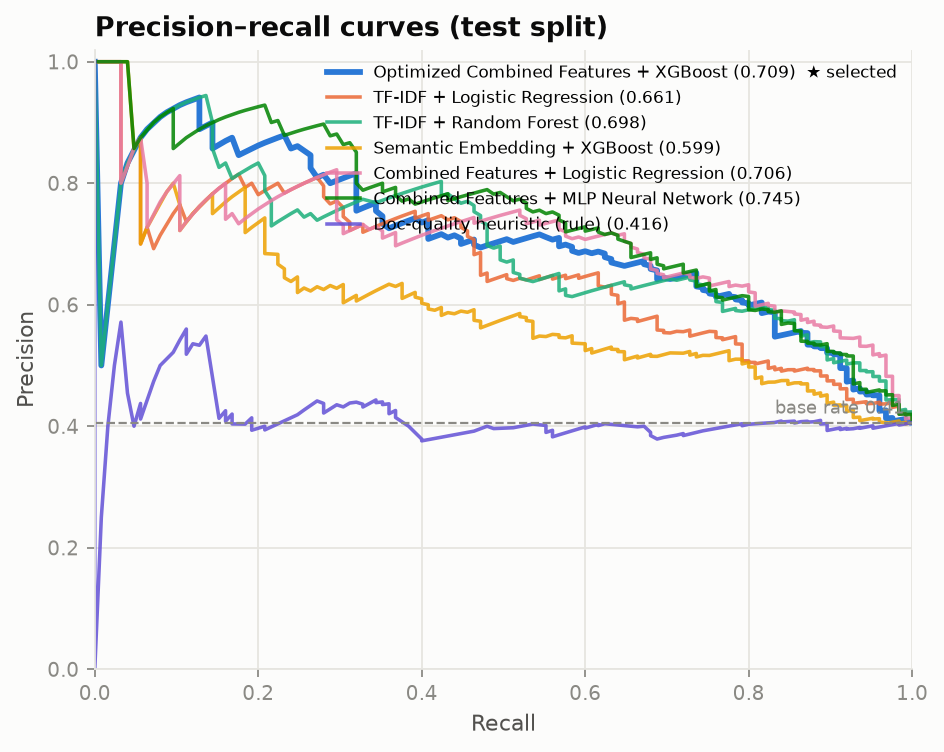
\includegraphics[width=\columnwidth]{03_pr_curves.png}\caption{Precision--recall curves on the test split; the dashed line is the failure base rate (no-skill).}\label{fig:pr}\end{figure}

\textbf{Confusion matrix.} On the 308 test tools the model produces TP 92, TN 131, FP 52 and FN 33 (Fig.~\ref{fig:cm}). Recall is favoured by design: a missed failure ships a broken tool to agents, whereas a false alarm only costs a documentation review.

\textbf{Ablation.} Table~\ref{tab:abl} trains XGBoost on each feature family and on combinations. All features reach CV PR-AUC 0.690, against 0.656 for the best single family (Text (LSA) + Lexical / naming), a gain of +0.033: text, semantic and structural signals are complementary.

\begin{table*}[t]\centering\caption{Feature-family ablation (XGBoost, 5-fold grouped CV on train+val; test PR-AUC for reference)}\label{tab:abl}
\resizebox{\textwidth}{!}{\begin{tabular}{llrlrr}\toprule
\textbf{Set} & \textbf{Families} & \textbf{\#feat} & \textbf{CV PR-AUC} & \textbf{CV ROC-AUC} & \textbf{Test PR-AUC} \\ \midrule
A & Text (LSA) + Lexical / naming & 89 & 0.656 ± 0.051 & 0.729 & 0.656 \\
B & Schema structure & 26 & 0.643 ± 0.034 & 0.697 & 0.640 \\
C & Semantic embedding & 48 & 0.619 ± 0.056 & 0.710 & 0.599 \\
D & Text (LSA) + Lexical / naming + Schema structure & 115 & 0.684 ± 0.041 & 0.752 & 0.694 \\
E & Semantic embedding + Schema structure & 74 & 0.664 ± 0.033 & 0.747 & 0.671 \\
F & Text (LSA) + Lexical / naming + Schema structure + Engineered risk scores + Semantic embedding & 169 & 0.690 ± 0.042 & 0.756 & 0.693 \\
\bottomrule\end{tabular}}\end{table*}

\textbf{Error analysis.} Most common source of model mistakes: missed failures whose dominant benchmark failure mode is invalid arg value (52\% of false negatives). The false negatives break down into Invalid arg value 52\%, Wrong tool selection 21\%, Missing required arg 15\%, Invalid arg type 6\%, Hallucinated parameter 6\%. Test outcomes — TP 92, TN 131, FP 52, FN 33. Hardest failure-mode slice: MISSING\_REQUIRED\_ARG (error rate 35\%, n=26). 79\% of false negatives are failure modes that depend on context outside the tool definition (argument values in the user request, sibling-tool routing, server strictness). False positives vs. true negatives: mean description length 14.75 vs 12.794 tokens; mean parameter count 3.481 vs 2.534. Table~\ref{tab:slice} slices the test errors by the dominant benchmark failure mode. Errors concentrate in failure modes that depend on information \emph{outside} the definition (the literal values a user types, sibling-tool routing), which bounds what any definition-only model can achieve.

\begin{table}[t]\centering\caption{Test errors by dominant failure mode (misclassification rate, positive rate, false negatives and false positives)}\label{tab:slice}
\resizebox{\columnwidth}{!}{\begin{tabular}{lrrrrr}\toprule
\textbf{Failure mode} & \textbf{n} & \textbf{Misclass.} & \textbf{Pos. rate} & \textbf{FN} & \textbf{FP} \\ \midrule
Invalid arg value & 139 & 31.6\% & 42\% & 17 & 27 \\
None & 68 & 22.1\% & 0\% & 0 & 15 \\
Wrong tool selection & 36 & 19.4\% & 92\% & 7 & 0 \\
Missing required arg & 26 & 34.6\% & 73\% & 5 & 4 \\
Invalid arg type & 15 & 33.3\% & 53\% & 2 & 3 \\
Hallucinated parameter & 12 & 25.0\% & 17\% & 2 & 1 \\
Invalid arg format & 9 & 22.2\% & 11\% & 0 & 2 \\
Schema parse error & 3 & 0.0\% & 100\% & 0 & 0 \\
\bottomrule\end{tabular}}\end{table}

\section{Conclusion \& Future Scope}
\textbf{Insights.} Tool-definition risk is learnable and explainable. A fused representation of text themes, semantics and schema structure clearly outperforms both a no-skill baseline and a documentation-quality heuristic, and the gain comes mainly from the representation rather than the choice of learner. SHAP turns each score into concrete fixes, such as documenting every parameter, adding formats and examples, and reducing nesting.

\textbf{Deployment considerations.} A FastAPI service validates every input (rejecting malformed JSON field by field), serves single and batch (CSV/JSON) prediction, health, metrics and SHAP endpoints, and a nine-page dashboard; descriptions are stored only as SHA-1 hashes. The service runs in a non-root Docker container with a health check, and is publicly deployed on Hugging Face Spaces at \url{https://nishanth0811-mcpguard.hf.space} (Gradio analyzer at \url{https://nishanth0811-mcpguard.hf.space/gradio}); the source code is at \url{https://github.com/NishanthAruchamy0927/MCPGuard}. Single-tool inference took about 40--110~ms on a CPU in our measurements and needs no LLM call.

\textbf{Limitations and future work.} Labels come from a calibrated \emph{simulated} agent rather than production telemetry, and the corpus is English and BFCL-heavy. Future work will (i) relabel with real LLM agents across several models (pass@$k$), (ii) add closed-loop LLM rewriting of risky descriptions verified by the risk model, (iii) fine-tune transformer encoders end-to-end, and (iv) integrate the scorer into MCP server CI pipelines.

\begin{thebibliography}{99}
\bibitem{mcp} Anthropic, ``Model Context Protocol specification,'' 2024. [Online]. Available: \url{https://modelcontextprotocol.io/specification}
\bibitem{mcpsurvey} X.~Hou, Y.~Zhao, S.~Wang, and H.~Wang, ``Model Context Protocol (MCP): Landscape, security threats, and future research directions,'' arXiv:2503.23278, 2025.
\bibitem{toolformer} T.~Schick, J.~Dwivedi-Yu, R.~Dess\`{i}, R.~Raileanu, M.~Lomeli, L.~Zettlemoyer, N.~Cancedda, and T.~Scialom, ``Toolformer: Language models can teach themselves to use tools,'' in \emph{Advances in Neural Information Processing Systems (NeurIPS)}, 2023.
\bibitem{react} S.~Yao, J.~Zhao, D.~Yu, N.~Du, I.~Shafran, K.~Narasimhan, and Y.~Cao, ``ReAct: Synergizing reasoning and acting in language models,'' in \emph{Proc. Int. Conf. Learning Representations (ICLR)}, 2023.
\bibitem{toolllm} Y.~Qin \emph{et al.}, ``ToolLLM: Facilitating large language models to master 16000+ real-world APIs,'' arXiv:2307.16789, 2023.
\bibitem{gorilla} S.~G. Patil, T.~Zhang, X.~Wang, and J.~E. Gonzalez, ``Gorilla: Large language model connected with massive APIs,'' arXiv:2305.15334, 2023.
\bibitem{bfcl} Gorilla LLM team, ``Berkeley Function-Calling Leaderboard (BFCL) dataset,'' Hugging Face, 2024. [Online]. Available: \url{https://huggingface.co/datasets/gorilla-llm/Berkeley-Function-Calling-Leaderboard}
\bibitem{hsieh} C.-Y. Hsieh, S.-A. Chen, C.-L. Li, Y.~Fujii, A.~Ratner, C.-Y. Lee, R.~Krishna, and T.~Pfister, ``Tool documentation enables zero-shot tool-usage with large language models,'' arXiv:2308.00675, 2023.
\bibitem{easytool} S.~Yuan, K.~Song, J.~Chen, X.~Tan, Y.~Shen, R.~Kan, D.~Li, and D.~Yang, ``EasyTool: Enhancing LLM-based agents with concise tool instruction,'' arXiv:2401.06201, 2024.
\bibitem{xgb} T.~Chen and C.~Guestrin, ``XGBoost: A scalable tree boosting system,'' in \emph{Proc. 22nd ACM SIGKDD Int. Conf. Knowledge Discovery and Data Mining}, 2016, pp. 785--794.
\bibitem{lgbm} G.~Ke, Q.~Meng, T.~Finley, T.~Wang, W.~Chen, W.~Ma, Q.~Ye, and T.-Y. Liu, ``LightGBM: A highly efficient gradient boosting decision tree,'' in \emph{Advances in Neural Information Processing Systems (NeurIPS)}, 2017, pp. 3146--3154.
\bibitem{sbert} N.~Reimers and I.~Gurevych, ``Sentence-BERT: Sentence embeddings using Siamese BERT-networks,'' in \emph{Proc. EMNLP-IJCNLP}, 2019, pp. 3982--3992.
\bibitem{minilm} W.~Wang, F.~Wei, L.~Dong, H.~Bao, N.~Yang, and M.~Zhou, ``MiniLM: Deep self-attention distillation for task-agnostic compression of pre-trained transformers,'' in \emph{Advances in Neural Information Processing Systems (NeurIPS)}, 2020.
\bibitem{umap} L.~McInnes, J.~Healy, and J.~Melville, ``UMAP: Uniform manifold approximation and projection for dimension reduction,'' arXiv:1802.03426, 2018.
\bibitem{optuna} T.~Akiba, S.~Sano, T.~Yanase, T.~Ohta, and M.~Koyama, ``Optuna: A next-generation hyperparameter optimization framework,'' in \emph{Proc. 25th ACM SIGKDD Int. Conf. Knowledge Discovery and Data Mining}, 2019, pp. 2623--2631.
\bibitem{shap} S.~M. Lundberg and S.-I. Lee, ``A unified approach to interpreting model predictions,'' in \emph{Advances in Neural Information Processing Systems (NeurIPS)}, 2017, pp. 4765--4774.
\bibitem{sklearn} F.~Pedregosa \emph{et al.}, ``Scikit-learn: Machine learning in Python,'' \emph{J. Mach. Learn. Res.}, vol.~12, pp. 2825--2830, 2011.
\bibitem{davis} J.~Davis and M.~Goadrich, ``The relationship between precision-recall and ROC curves,'' in \emph{Proc. 23rd Int. Conf. Machine Learning (ICML)}, 2006, pp. 233--240.
\bibitem{saito} T.~Saito and M.~Rehmsmeier, ``The precision-recall plot is more informative than the ROC plot when evaluating binary classifiers on imbalanced datasets,'' \emph{PLoS ONE}, vol.~10, no.~3, e0118432, 2015.
\bibitem{efron} B.~Efron and R.~J. Tibshirani, \emph{An Introduction to the Bootstrap}. New York, NY, USA: Chapman \& Hall, 1993.
\end{thebibliography}
\end{document}
